\documentclass[11pt]{article}

% Font
\usepackage[T1]{fontenc}
\usepackage{palatino}
\usepackage{microtype}

% Layout
\usepackage{geometry}
\geometry{margin=1in, top=1.2in, bottom=1.2in}

% Spacing
\usepackage{setspace}
\onehalfspacing

% Graphics & figures
\usepackage{graphicx}
\usepackage{float}
\usepackage{subcaption}
\usepackage[labelfont=bf, font=small, skip=6pt]{caption}

% Math
\usepackage{amsmath}
\usepackage{amssymb}
\usepackage{amsthm}

% Tables
\usepackage{booktabs}
\usepackage{multirow}
\usepackage{array}
\renewcommand{\arraystretch}{1.3}

% Code listings
\usepackage{listings}
\usepackage{xcolor}

% Section styling
\usepackage{titlesec}
\titleformat{\section}{\large\bfseries}{\thesection.}{0.5em}{}[\titlerule]
\titleformat{\subsection}{\normalsize\bfseries}{\thesubsection.}{0.5em}{}
\titlespacing{\section}{0pt}{1.5em}{0.8em}
\titlespacing{\subsection}{0pt}{1em}{0.4em}

% Header & footer
\usepackage{fancyhdr}
\pagestyle{fancy}
\fancyhf{}
\rhead{\small\textit{Reproduction Study: HyperTurtle}}
\lhead{\small\textit{Manoj Khatri}}
\cfoot{\thepage}
\renewcommand{\headrulewidth}{0.4pt}

% Hyperlinks
\usepackage{hyperref}
\hypersetup{
    colorlinks=true,
    linkcolor=black,
    citecolor=black,
    urlcolor=blue
}

\title{Reproducing HyperTurtle: Accelerating Nested Virtualization with Hyperupcalls}
\author{Manoj Khatri}
\date{April 2026}

\begin{document}

\maketitle


\begin{abstract}
This report reproduces the primary results of the USENIX ATC 2025 paper \textit{Accelerating Nested Virtualization with HyperTurtle} on two CloudLab c220g5 nodes. HyperTurtle offloads L1 hypervisor logic into L0 as eBPF programs across three subsystems: EPT fault handling, networking, and profiling. All three subsystems ran successfully. On EPT, HyperTurtle reduced median L2 fault latency from 23.43\,$\mu$s to 5.55\,$\mu$s, a 4.22$\times$ speedup, and improved Kata startup time by 20--33\% across six images. Networking and profiling also reproduce the paper's main claims: HyperTurtle network functions stay close to the fast path and substantially outperform the nested baseline, and profiling overhead at 1\,kHz is substantially lower than with conventional L1 profiling.
\end{abstract}

\section{Introduction}

Nested virtualization lets a guest VM run its own hypervisor and manage further VMs, which is the basis of VM-based container deployments such as Kata Containers, but its main weakness is performance. Every L2 event requiring hypervisor intervention must pass through both the guest hypervisor (L1) and the bare-metal hypervisor (L0), creating multiple world switches per event. The paper quantifies this cost: each world switch takes roughly 1\,$\mu$s and accounts for about 33\% of total vm-exit handling time. On the EPT fault path a single L2 fault requires six world switches against two in the non-nested case, producing more than a 5$\times$ average-latency increase and a substantial increase in Kata container boot time.

HyperTurtle reduces this overhead without removing L1 from control of L2. Its key mechanism is the \emph{hyperupcall}: a small eBPF program encapsulating a fragment of L1 hypervisor logic that executes in the L0 context when an L2 vm-exit occurs, eliminating the world switches for that event. Because hyperupcalls run through the kernel's existing eBPF verifier, they require only modest changes to L0 KVM and QEMU and no modifications to L2. The paper applies this to three subsystems: EPT fault handling, L1-controlled network I/O, and application profiling, and reports substantial gains in all three.

This report reproduces those results using the authors' public repository (\url{https://github.com/acsl-technion/hyperturtle}) on two CloudLab c220g5 nodes in the same Intel Skylake-SP CPU family as the paper's hardware. The target experiments are EPT fault latency and Kata startup, network performance, and profiling overhead. The repository contains only build instructions. The authors provided a VM launch script on request, which required further modification. All remaining evaluation infrastructure was written from scratch, and substantial code-level fixes were required before any experiment could run. The EPT path in particular required fixing several prototype bugs and making the boot sequence deterministic before results matched the paper.

\section{Experimental Setup}

\subsection{Hardware}

I ran the evaluation on two CloudLab c220g5 nodes (Figure~\ref{fig:hardware}). Hardware differences from the paper are summarised in Table~\ref{tab:hardware}. Both CPU models belong to the Skylake-SP family with 46-bit physical addressing, making this a reasonable platform for trend-level comparison. One node was the nested-virtualization host running L0, L1, and L2, and the second acted as the benchmark client for networking experiments.

\begin{table}[H]
    \centering
    \caption{Hardware differences between the paper and this setup (common factors: Skylake-SP family, 46-bit physical addressing, SMT off).}
    \label{tab:hardware}
    \begin{tabular}{lll}
        \toprule
        Component & Paper & This setup \\
        \midrule
        CPU model & 2$\times$ Xeon Silver 4216 & 2$\times$ Xeon Silver 4114 \\
        Cores per NUMA node & 16 & 10 \\
        CPU base clock & 2.1\,GHz & 2.2\,GHz \\
        L3 cache & 22\,MB & 13.75\,MB \\
        RAM & 512\,GiB & $\sim$192\,GiB \\
        NIC & Nvidia MT27710 (ConnectX-4) & Intel X520/X540 \\
        NIC link speed & 25\,GbE & 10\,GbE \\
        \bottomrule
    \end{tabular}
\end{table}

\begin{figure}[H]
    \centering
    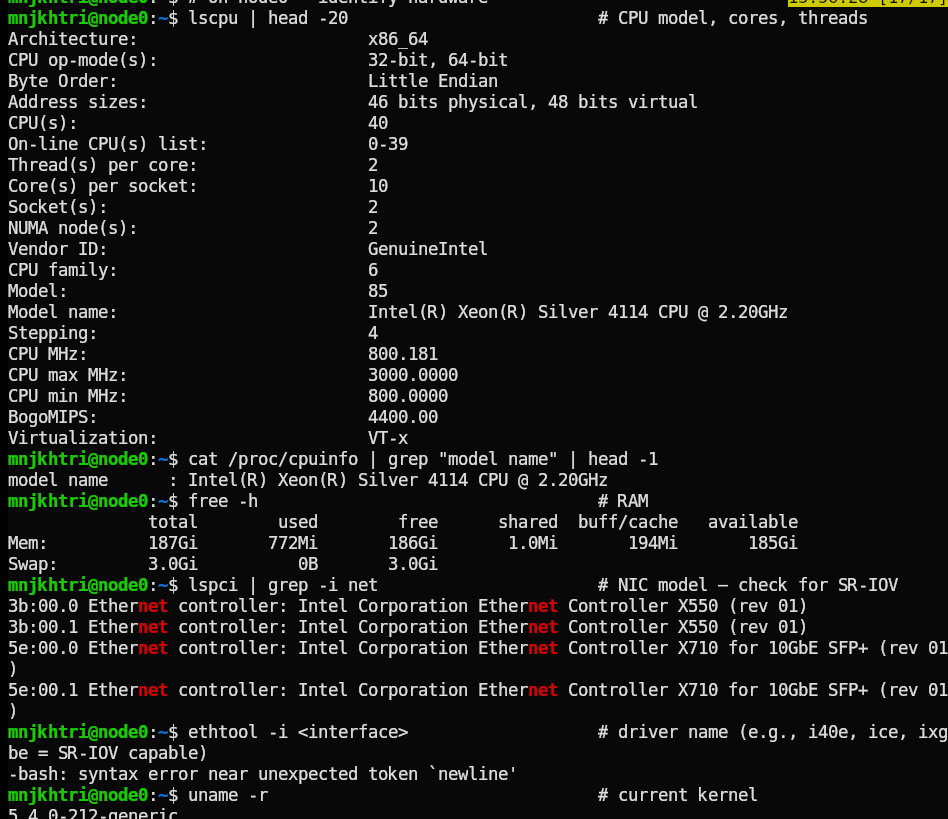
\includegraphics[width=0.5\linewidth]{figures/l0_hardware_spec.png}
    \caption{L0 host hardware: Xeon Silver 4114, 46-bit physical addressing, approximately 187\,GiB visible memory, and Intel X550/X710 network devices.}
    \label{fig:hardware}
\end{figure}

\subsection{Software Stack}

I built the software stack from the authors' public HyperTurtle repository, which contains the modified Linux kernel, QEMU tree, and hyperupcall implementations. The L0 host ran Ubuntu 20.04.6 with the HyperTurtle Linux 5.16.0+ kernel and HyperTurtle QEMU 7.2.0. libbpf was built from the HyperTurtle Linux tree, with the QEMU source modified accordingly. The L1 guest ran Ubuntu 20.04.6 with the same kernel, 12 vCPUs, and 64\,GiB of RAM. A 9p shared folder mounted the artifact tree from L0 into L1, allowing kernel sources, headers, and scripts to be shared without duplication. L2 guests ran as Kata Containers 3.2.0 with the bundled Kata guest kernel 6.1.38, with the active hypervisor configuration adjusted as needed during setup and evaluation.

\textbf{Steps not covered by the artifact.} Beyond a single L1 launch script (\texttt{run\_virt\_host}) and manual steps for attaching a networking hyperupcall, the repository provides no evaluation infrastructure. All benchmark drivers, measurement harnesses, Kata startup scripts, NGINX/Memcached/Redis load configurations, and profiling pipelines were written from scratch. Several code-level fixes were also required before any experiment could run:

\begin{itemize}
    \item \textbf{Missing QEMU\_CR3 injection}: the guest page-table root was not being exported into the shared eBPF state, so the EPT bypass could not resolve mappings correctly.
    \item \textbf{MAPS\_DEV\_OFFSET incorrect}: the value was 5 in \texttt{kvm\_host.h} but must be 1. With the wrong value all shared maps were NULL and the hyperupcall was non-functional.
    \item \textbf{Hot-path \texttt{pr\_err} calls}: five diagnostic prints in \texttt{arch/x86/kvm/x86.c} fired on every shared-memory EPT page fault, flooding the serial console and extending container boot times to over 23\,s. All were commented out.
    \item \textbf{Exporter race during boot}: the original \texttt{ept\_fault.guest} loop disabled the bypass during Docker/Kata process transitions. The fix used a temporary sticky-mode workaround together with a split create/start boot protocol.
    \item \textbf{Missing memory preallocation}: the final EPT path required preallocated guest memory so the exporter could populate the shared maps before the L2 guest started faulting pages.
    \item \textbf{Broken firewall sources}: the \texttt{packet\_filter} sources in the repository snapshot had type errors and could not be built, so they were replaced with a minimal stateless XDP filter.
    \item \textbf{CPU pinning}: the HyperTurtle profiling path samples a fixed host CPU, so the hot outer L1 QEMU thread was pinned to host CPU 5 with \texttt{taskset} before each profiling run.
\end{itemize}

\subsection{VM Configuration and Boot Parameters}

Both L0 and L1 were booted with \texttt{idle=poll} and \texttt{nopti}. On L0, SMT was disabled, nested KVM was enabled, \texttt{ple\_gap} was set to 0, and vhost-net zero-copy transmit was enabled. The \texttt{idle=poll} flag on L1 proved critical: without it, EPT fault latency appeared artificially low and inconsistent with the paper's numbers. For the final EPT runs, the Kata configuration also used synchronous fault handling and guest-memory preallocation so that the exporter and bypass maps were populated before the L2 guest booted.

For networking, L1 was booted without \texttt{intel\_iommu=on}. Including it caused DMAR faults on the virtio NIC path even without any hyperupcall attached, which invalidated all early networking measurements.

For profiling, Kata's default \texttt{cpu\_features="pmu=off"} was changed to \texttt{pmu=on}, as the default configuration exposed no performance counters inside L2.

\section{Methodology}

\subsection{EPT}

The EPT latency microbenchmark allocated anonymous memory with \texttt{mmap} and touched each 4\,KiB page once, measuring per-fault latency via \texttt{rdtsc}. For the Figure~9a result, the benchmark ran inside an L2 Kata container with the \texttt{ept\_fault} hyperupcall loaded, the exporter started first, and \texttt{kvm-intel} reloaded so that the shared PCI-backed maps were discovered correctly. The non-nested reference run was collected directly inside L1.

For container startup, the protocol split launch into \texttt{docker create}, a short wait for the exporter to discover the L2 VMM and populate the maps, and then \texttt{docker start}. Six container images were tested (Alpine, Ubuntu, Java, JavaScript, Python, and a persistent-data variant), and startup time was measured until the containerised application responded over the network.

\subsection{Networking}

The networking evaluation targeted Table~7, Figures~12a/12b, and Figure~13. The benchmark datapath ran over L1 \texttt{enp1s0f0} through L0 tap device \texttt{tap1} to bridge \texttt{br0} at \texttt{10.10.1.0/24}. A key early finding was that HyperTurtle's QEMU networking code resolves a \emph{guest netdev index} rather than a Linux ifindex, and the correct value for the benchmark NIC was netdev index 1. Four hyperupcall variants were validated and benchmarked: \texttt{pass}, \texttt{rate\_limiter}, \texttt{tcp\_top}, and a stateless XDP firewall. Stale \texttt{clsact} qdiscs and orphaned XDP links were removed before each run to prevent attachment failures.

For NGINX (Figure~12a), a tiny-response benchmark proved insensitive to networking differences and was replaced with a 64\,MiB static-file workload. For Memcached (Figure~13), the networking sweep used the custom benchmark driver developed for this reproduction to generate throughput-versus-p99 curves under the patched firewall. Absolute throughput values therefore reflect the chosen client, and the relative ordering across configurations is the primary comparison point.

\subsection{Profiling}

The profiling evaluation targeted Table~4 / Figure~9b and Figure~14. Three setup steps were required: exposing PMU counters inside Kata, building \texttt{mutilate} on L0 for Memcached load generation, and pinning the hot outer L1 QEMU thread to host CPU 5 because the HyperTurtle profiling path samples a fixed host CPU. Conventional L1 profiling was driven by a small helper based on \texttt{perf\_event\_open()}.

For Table~4 / Figure~9b, the L0\,$\to$\,L1 and HT\,$\to$\,L2 entries were measured with the L0 \texttt{function\_graph} tracer on the sampled CPU, while the L1\,$\to$\,L2 path was reconstructed from L0 KVM tracepoint bursts. The L1\,$\to$\,L1 case was not measured reliably because L1-local tracing misses time spent in L0 during the repeated world switches. For Figure~14, Memcached ran inside a Kata container and was loaded with \texttt{mutilate} using the Facebook ETC workload distribution. All runs used Nested-VirtIO networking, capping throughput at roughly 21\,Kops/s instead of the paper's 80\,Kops/s. Three lanes were compared at 1\,kHz and 4\,kHz: no profiling, conventional L1 profiling, and HyperTurtle profiling.

\section{Results}

\subsection{EPT Fault Handling}

HyperTurtle matches the paper's main EPT result. As shown in Table~\ref{tab:ept} and Figure~\ref{fig:ept_latency}, the nested baseline measured 23.43\,$\mu$s median fault latency, while HyperTurtle reduced that to 5.55\,$\mu$s, a 4.22$\times$ speedup. The HyperTurtle median is within 0.92\,$\mu$s of the non-nested L1 reference at 4.63\,$\mu$s, showing that the bypass reaches near-native latency under correct initialization.

\begin{table}[H]
    \centering
    \caption{Final EPT fault microbenchmark results.}
    \label{tab:ept}
    \begin{tabular}{lcccc}
        \toprule
        Configuration & Average ($\mu$s$)$ & Median ($\mu$s$)$ & 99p ($\mu$s$)$ & 99.9p ($\mu$s$)$ \\
        \midrule
        L1 VM (non-nested) & 5.02 & 4.63 & 9.48 & 46.75 \\
        L2 VM baseline & 22.33 & 23.43 & 52.16 & 73.67 \\
        L2 VM + HyperTurtle & 8.31 & 5.55 & 17.72 & 988.29 \\
        \bottomrule
    \end{tabular}
\end{table}

\begin{figure}[H]
    \centering
    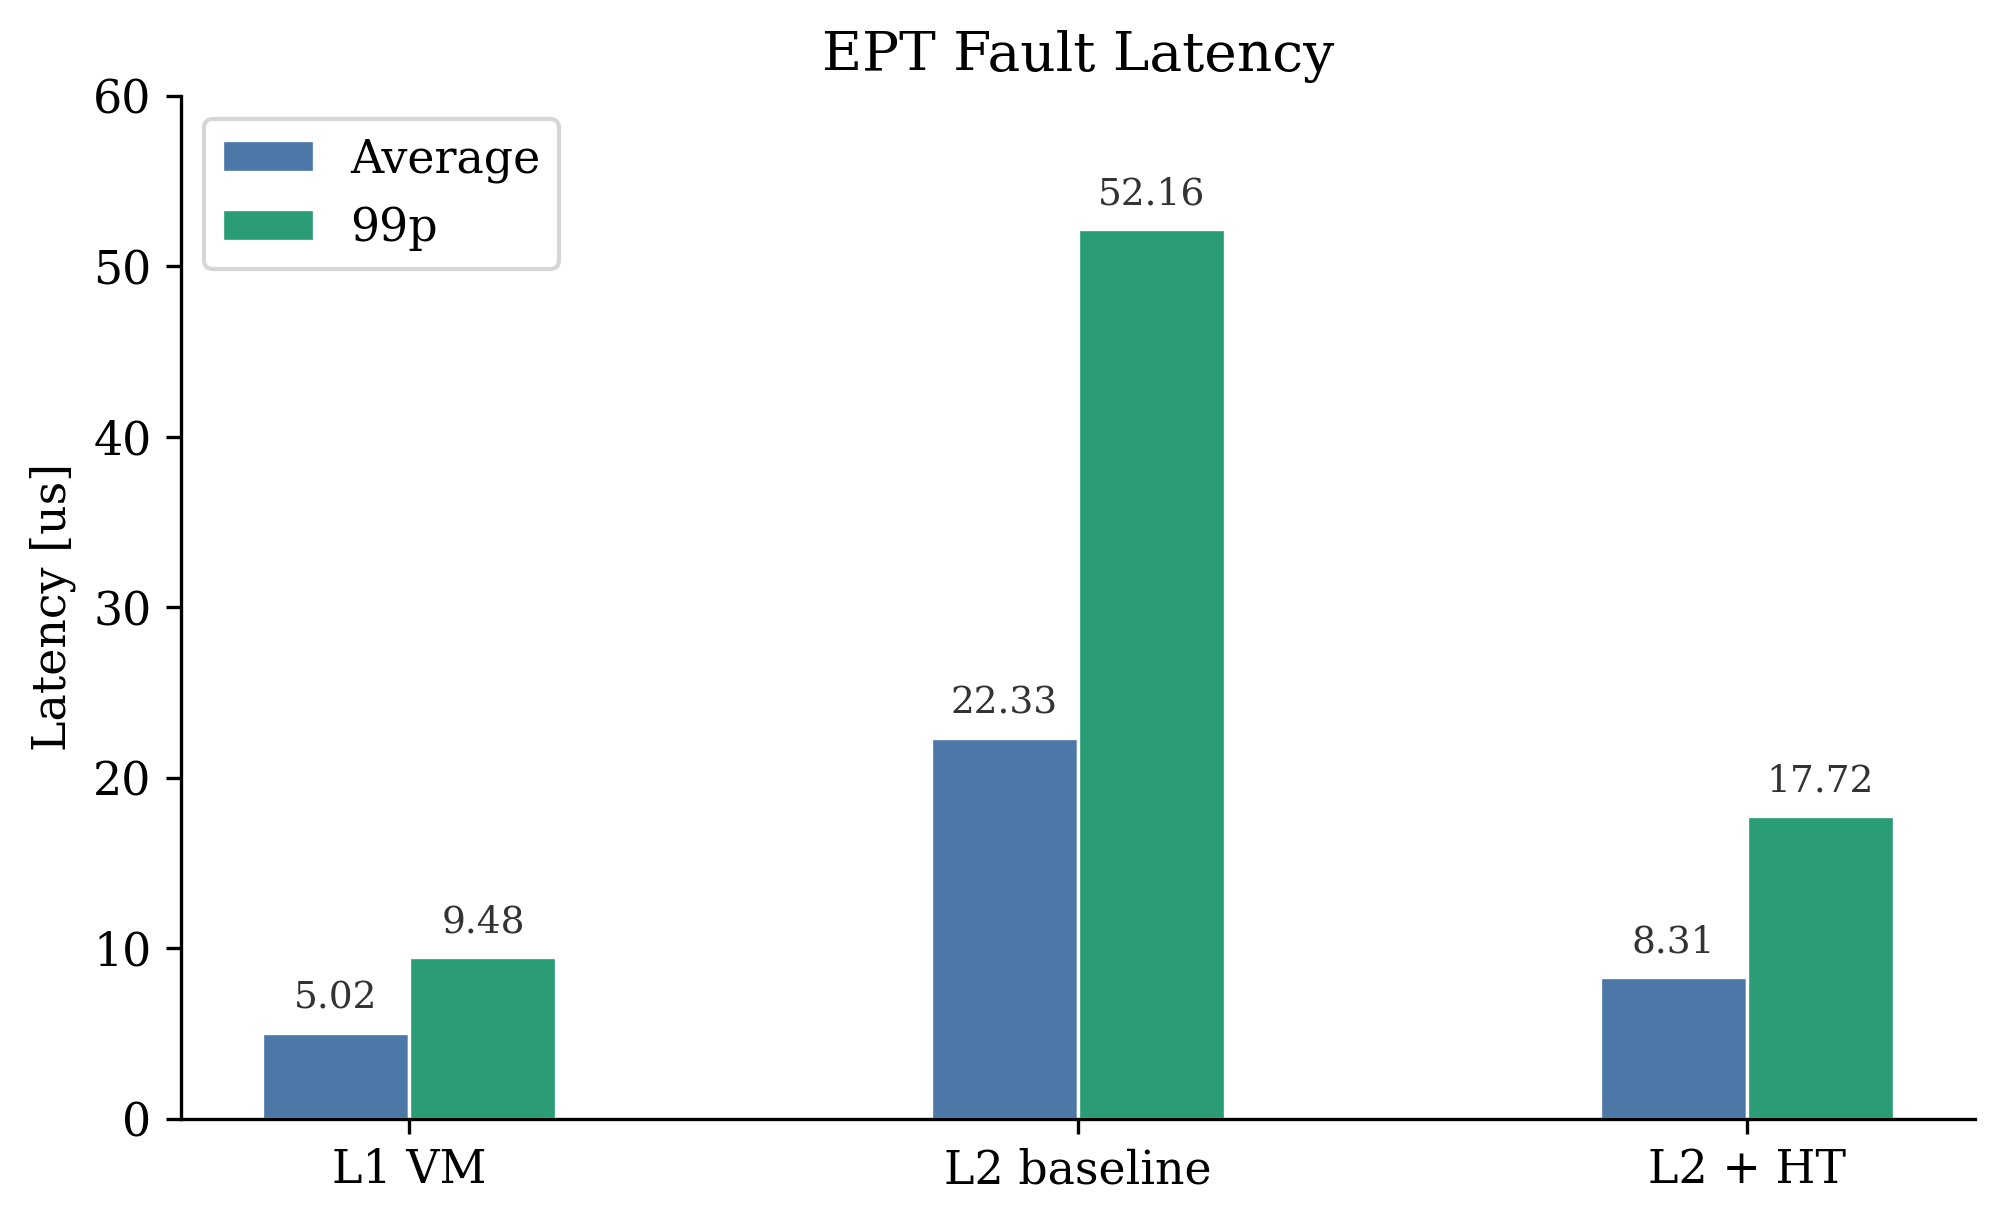
\includegraphics[width=0.5\linewidth]{figures/ept_latency_reproduction.png}
    \caption{EPT fault latency. HyperTurtle reduces nested L2 fault latency to near-native L1 levels.}
    \label{fig:ept_latency}
\end{figure}

\begin{figure}[H]
    \centering
    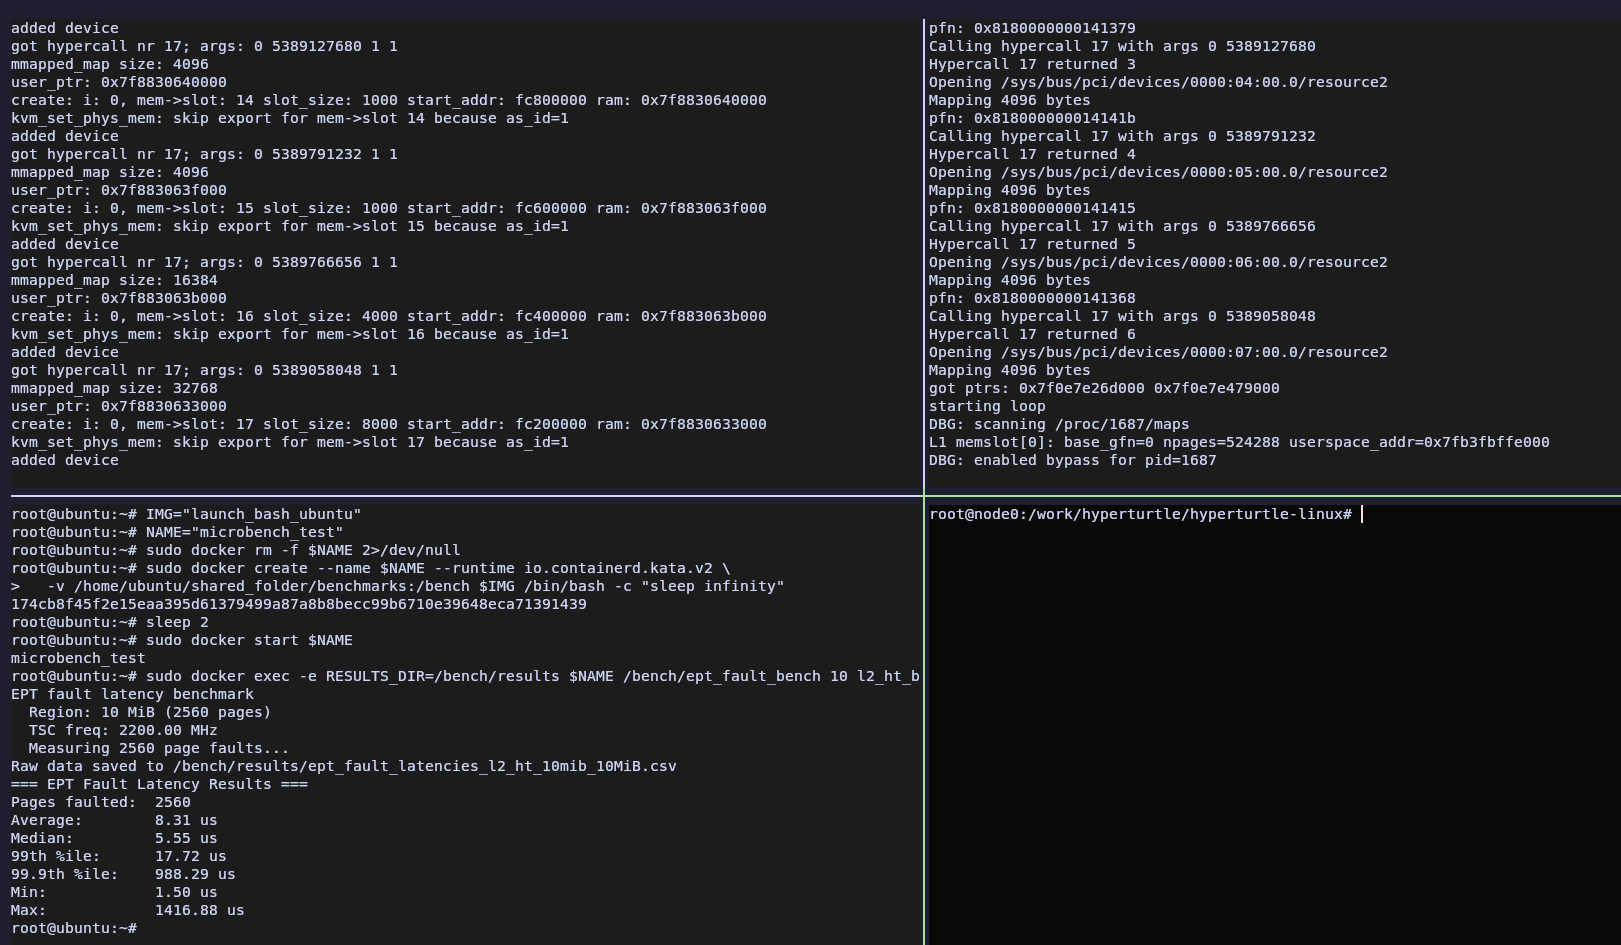
\includegraphics[width=0.7\linewidth]{figures/ept_benchmark_final_run.png}
    \caption{Terminal output from the final EPT benchmark run. The left pane shows the exporter discovering the L2 QEMU process and populating the shared maps. The right pane shows the benchmark result (median 5.55\,$\mu$s, 99p 17.72\,$\mu$s).}
    \label{fig:ept_bench}
\end{figure}

HyperTurtle also reduced container boot time across all six images (Table~\ref{tab:startup} and Figure~\ref{fig:kata_startup}), averaging 29\% faster and ranging from 20\% to 33\%, reflecting the reduced EPT fault overhead during the guest kernel's memory initialisation phase.

\begin{table}[H]
    \centering
    \caption{Final Kata startup times with the working EPT bypass path.}
    \label{tab:startup}
    \begin{tabular}{lccc}
        \toprule
        Image & Baseline (s) & HyperTurtle (s) & Speedup \\
        \midrule
        alpine & 2.88 & 2.072 & 28\% \\
        ubuntu & 2.77 & 1.857 & 33\% \\
        java & 2.76 & 1.949 & 29\% \\
        js & 2.65 & 2.127 & 20\% \\
        python & 2.68 & 1.893 & 29\% \\
        pd & 2.67 & 1.818 & 32\% \\
        Average & 2.74 & 1.95 & 29\% \\
        \bottomrule
    \end{tabular}
\end{table}

\begin{figure}[H]
    \centering
    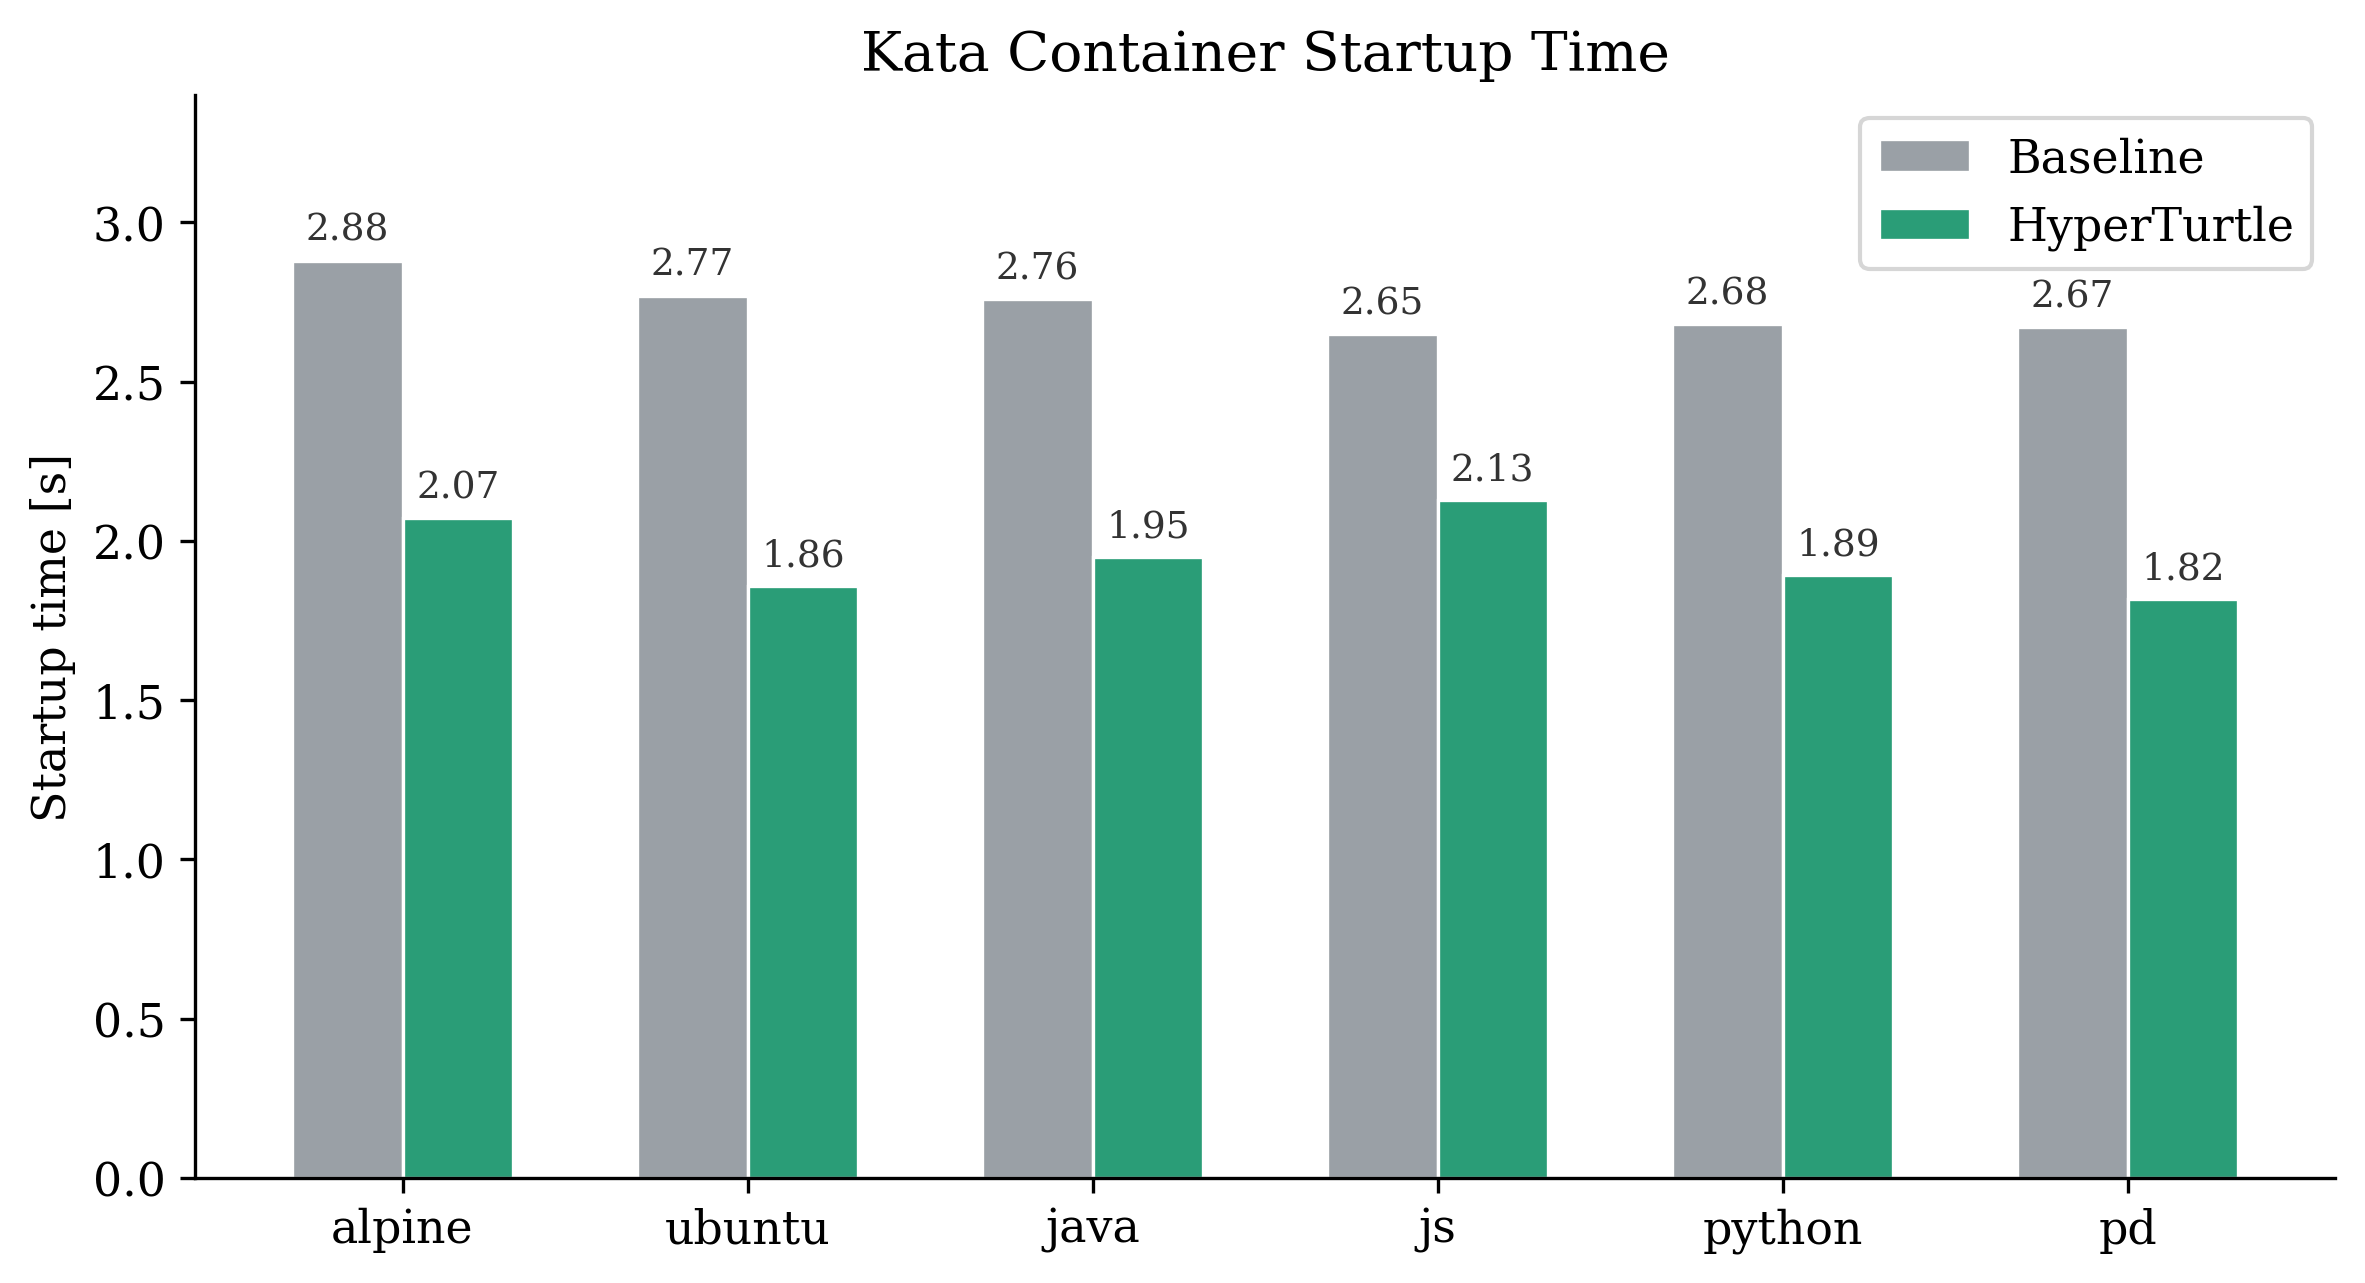
\includegraphics[width=0.6\linewidth]{figures/kata_startup_comparison.png}
    \caption{Kata container startup time by image. HyperTurtle reduces boot time by 20--33\% across all six images.}
    \label{fig:kata_startup}
\end{figure}


\subsection{Networking}

The networking results reproduce the paper's main ordering across configurations: HyperTurtle stays close to the fast path and substantially outperforms the nested baseline on network-sensitive workloads. Note that the paper used a 25\,GbE ConnectX-4 NIC whereas this setup is limited to 10\,GbE, so absolute throughput values are not directly comparable and the observed gains are likely conservative.

The clearest application-level result is the large-file NGINX benchmark (Figure~12a equivalent). As shown in Figure~\ref{fig:nginx}, when serving a 64\,MiB static file, the nested baseline achieved 1000.75\,MiB/s while plain HyperTurtle reached 1812.38\,MiB/s. The added network functions remained close to that fast path: \texttt{rate\_limiter} at 1641.41\,MiB/s and \texttt{tcp\_top} at 1706.01\,MiB/s. Figure~\ref{fig:rate_limiter} confirms the \texttt{rate\_limiter} hyperupcall was active and passing traffic at approximately 20\,Gbit/s. By contrast, the Redis GET benchmark corresponding to Figure~12b was largely flat on this setup: all four rows remained between 436 and 446\,MiB/s, so Redis did not expose a strong nested penalty here.

\begin{figure}[H]
    \centering
    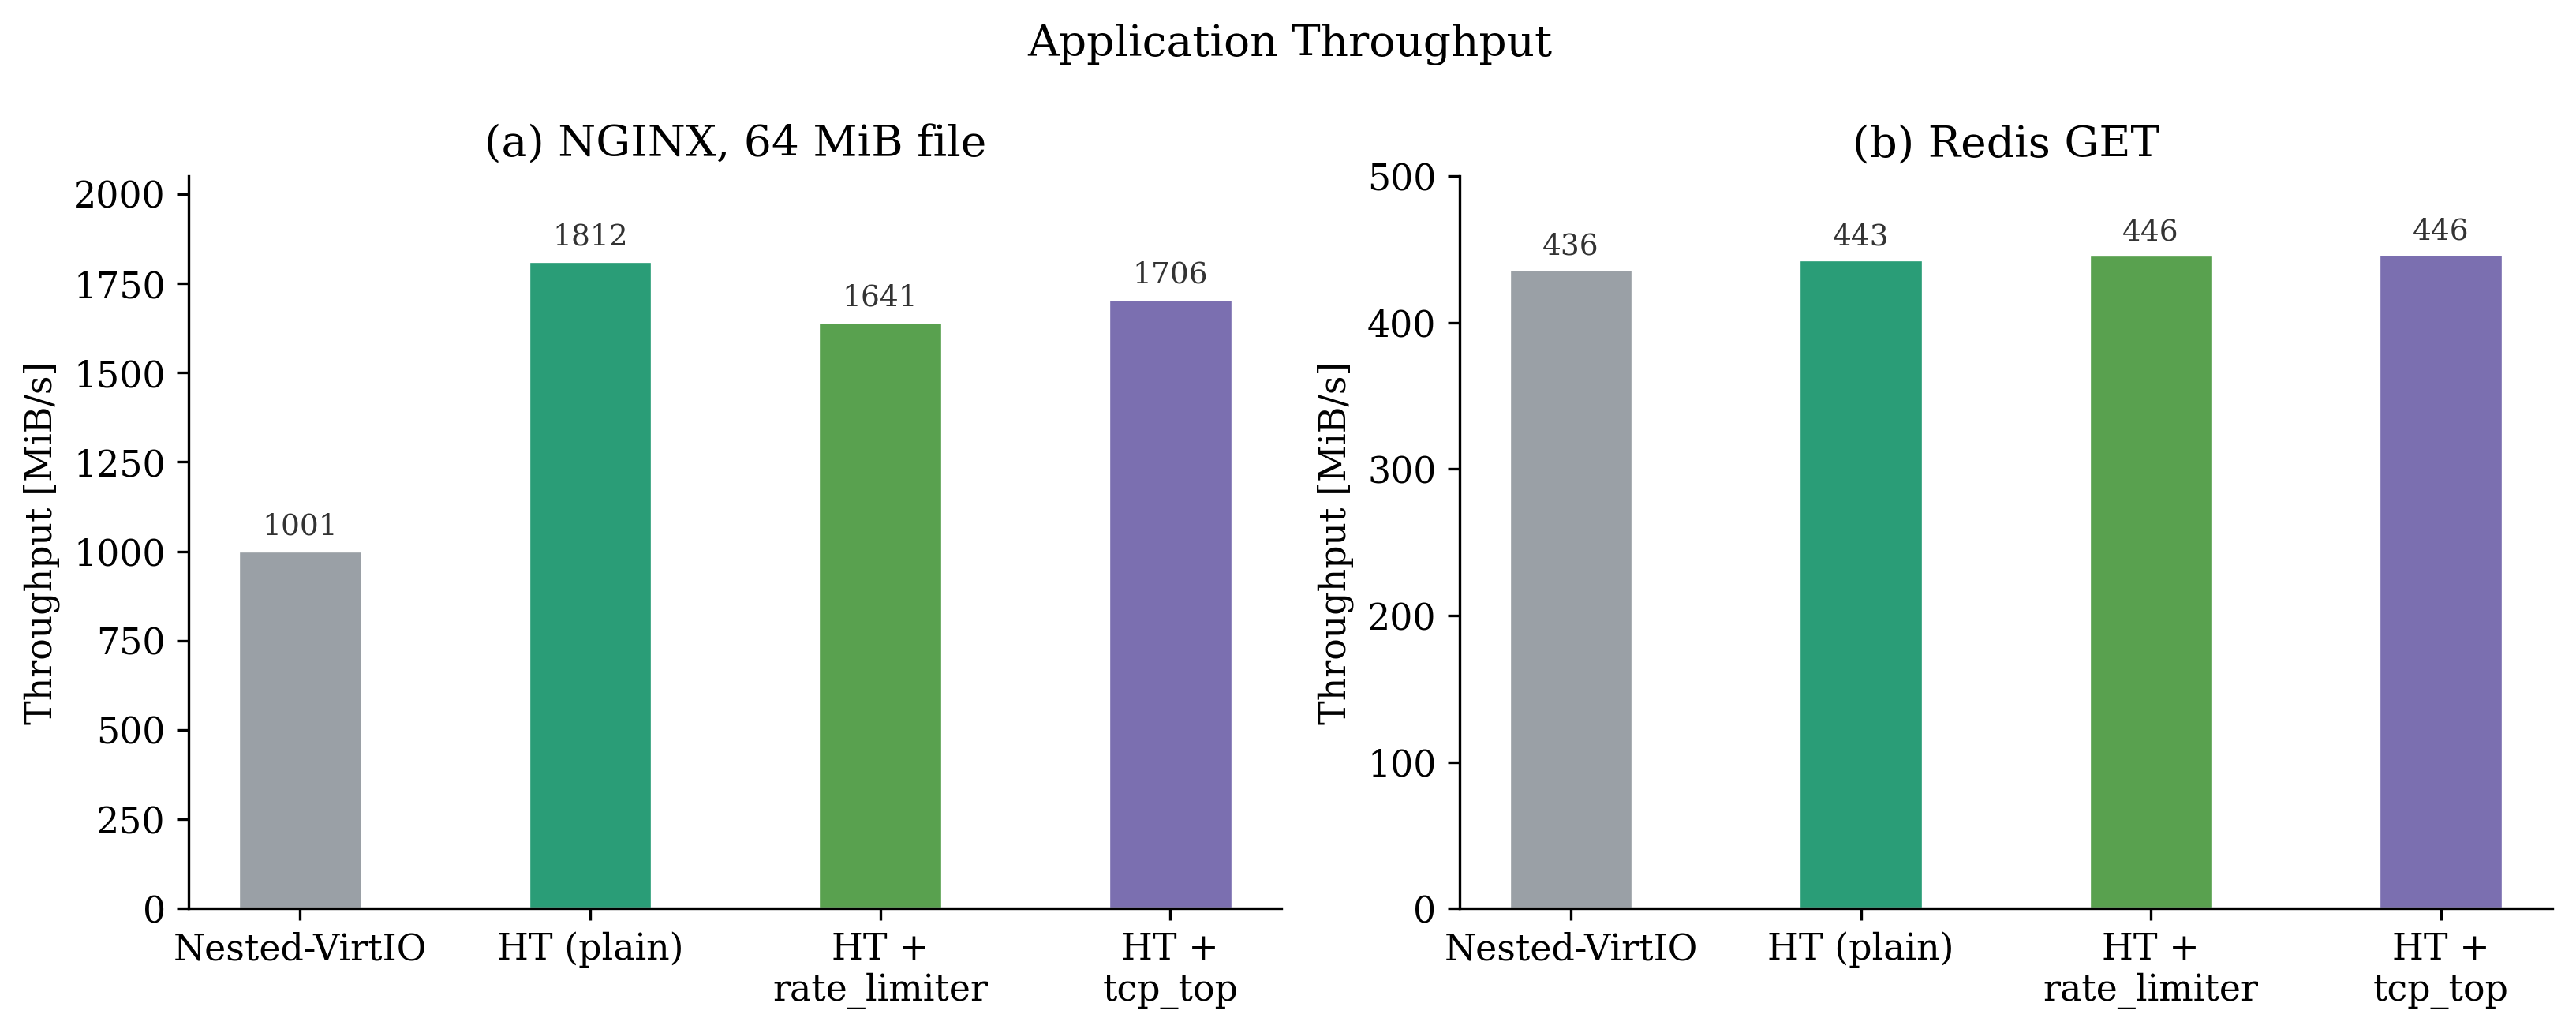
\includegraphics[width=0.9\linewidth]{figures/nginx_largefile_throughput.png}
    \caption{Application throughput. \textbf{(a) NGINX:} HyperTurtle stays well above the nested baseline even with active network functions. \textbf{(b) Redis:} all four configurations are close, making Redis an important negative result rather than a strong reproduction of the paper's Figure~12b gap.}
    \label{fig:nginx}
\end{figure}

\begin{figure}[H]
    \centering
    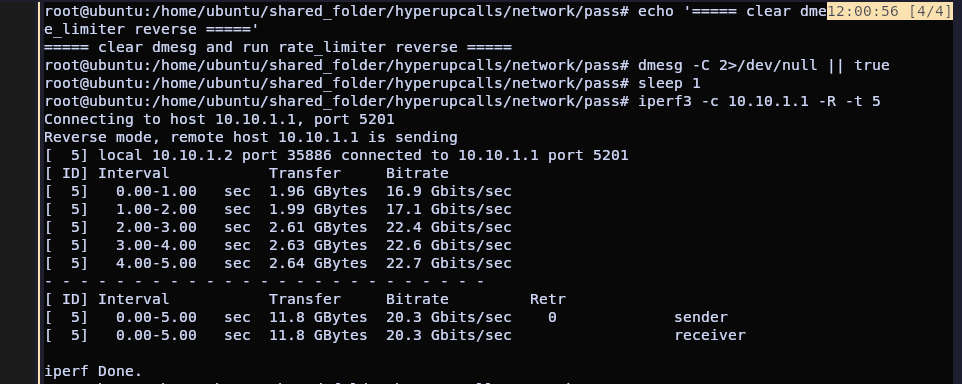
\includegraphics[width=0.5\linewidth]{figures/network_rate_limiter_reverse_iperf.png}
    \caption{iperf3 reverse throughput with the \texttt{rate\_limiter} hyperupcall attached, confirming the function was active and passing traffic at approximately 20\,Gbit/s.}
    \label{fig:rate_limiter}
\end{figure}

The Memcached-under-firewall experiment best captures the Figure~13 trend. Figure~\ref{fig:memcached} and Table~\ref{tab:netops} show that at the 500\,$\mu$s p99 target, HyperTurtle with the patched firewall sustained substantially more throughput than the nested baseline with firewall, a 26\% advantage at the nearest comparable operating point. A no-firewall plain HyperTurtle run reached a very similar point, confirming that the firewall itself imposed only a modest additional cost, consistent with the paper's claim. Figure~\ref{fig:firewall_loaded} confirms the firewall hyperupcall was successfully loaded during these runs.

\begin{figure}[H]
    \centering
    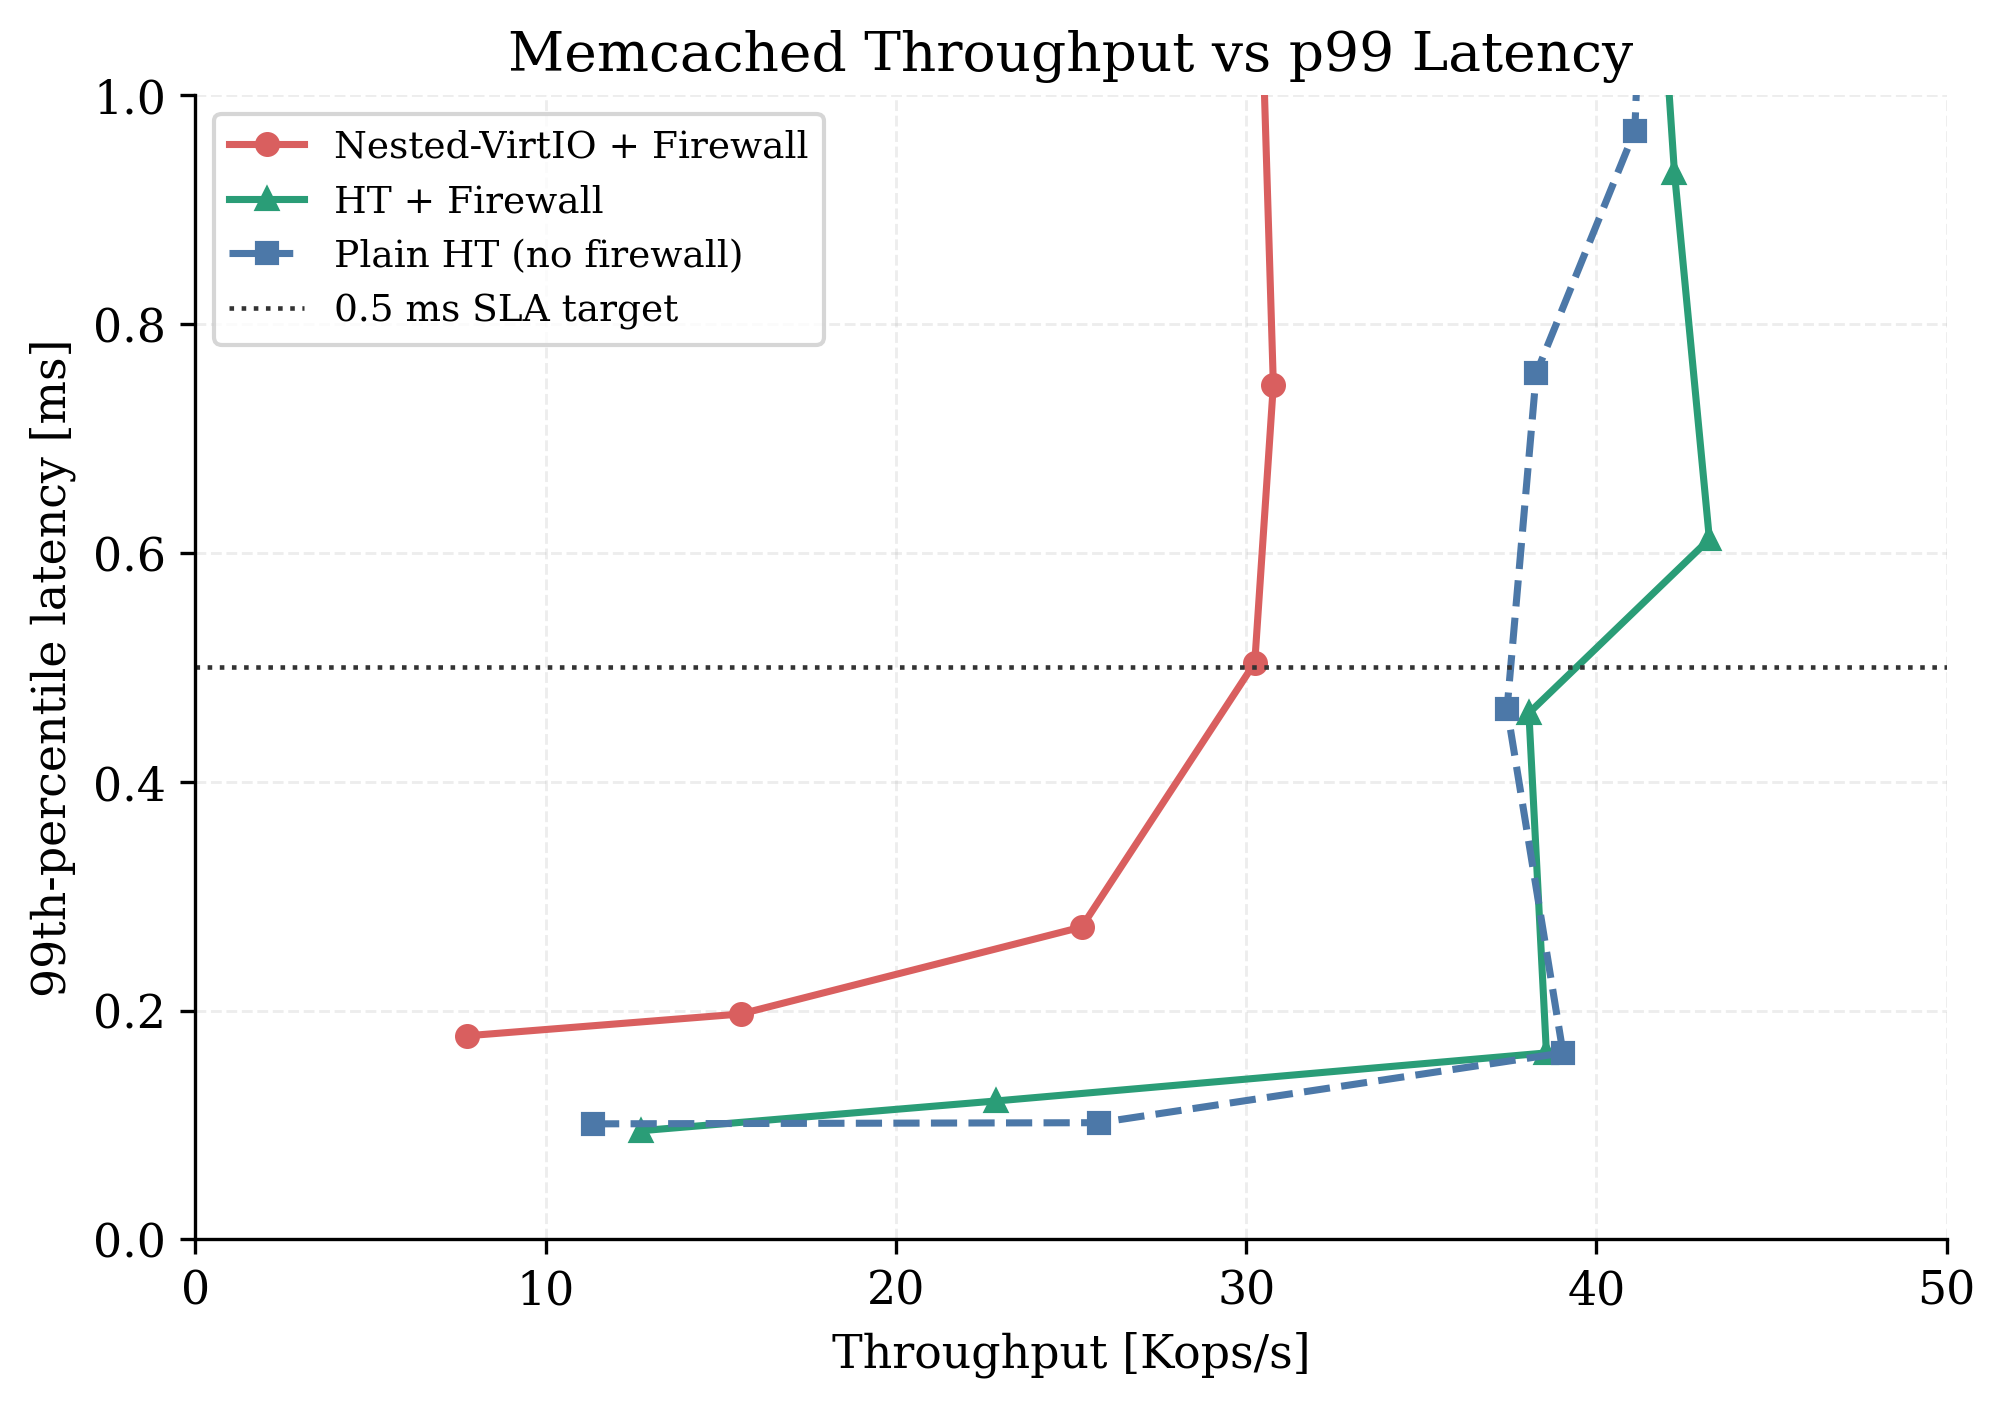
\includegraphics[width=0.5\linewidth]{figures/memcached_firewall_curve.png}
    \caption{Memcached throughput versus 99th-percentile latency. HyperTurtle with firewall support sustains substantially more throughput than the nested baseline near the 500\,$\mu$s target.}
    \label{fig:memcached}
\end{figure}

\begin{figure}[H]
    \centering
    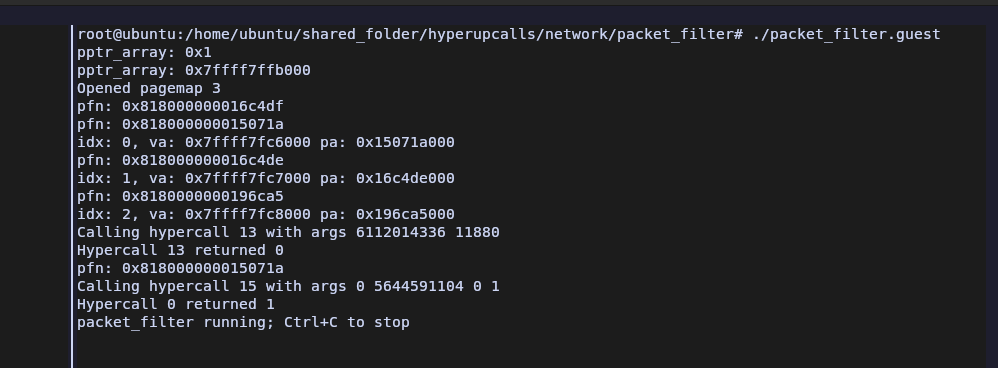
\includegraphics[width=0.5\linewidth]{figures/network_firewall_hyperupcall_loaded.png}
    \caption{Terminal output confirming the firewall hyperupcall loaded and linked successfully during the Memcached experiments.}
    \label{fig:firewall_loaded}
\end{figure}

\begin{table}[H]
    \centering
    \caption{Networking operating-point comparison near the 500\,$\mu$s p99 target.}
    \label{tab:netops}
    \begin{tabular}{lccc}
        \toprule
        Configuration & Throughput (Kops/s) & p99 ($\mu$s) & Relative \\
        \midrule
        Nested-VirtIO + Firewall & 30.25 & 504 & 1.00$\times$ \\
        HyperTurtle + Firewall & 38.07 & 460 & 1.26$\times$ \\
        Plain HyperTurtle (no firewall) & 37.45 & 464 & 1.24$\times$ \\
        \bottomrule
    \end{tabular}
\end{table}

Table~\ref{tab:net7} shows the Table~7 proxy: the nested baseline reached 10.61\,Gb/s while HyperTurtle + Pass and HyperTurtle + Firewall reached 19.40 and 18.73\,Gb/s respectively, capturing the correct ordering. A Direct Assignment row was not included because VFIO device assignment could not be configured under the default Kata QEMU setup.

\begin{table}[H]
    \centering
    \caption{Table~7 proxy from the networking experiments.}
    \label{tab:net7}
    \begin{tabular}{lcc}
        \toprule
        Configuration & Throughput (Gb/s) & Avg.\ latency ($\mu$s) \\
        \midrule
        Nested-VirtIO & 10.61 & N/A \\
        HyperTurtle + Pass & 19.40 & 59.87 \\
        HyperTurtle + Firewall & 18.73 & 59.80 \\
        \bottomrule
    \end{tabular}
\end{table}

\subsection{Profiling}

The profiling path worked correctly once the hot outer L1 QEMU thread was pinned to host CPU 5: the \texttt{rbp\_traces} map advanced at 1{,}000.3\,Hz during live Kata execution, confirming that HyperTurtle profiling was active. Three of the four Table~4 / Figure~9b entries were measured. As shown in Figure~\ref{fig:sampling_latency}, L0\,$\to$\,L1 measured 4.93\,$\mu$s against the paper's 5.66\,$\mu$s, HT\,$\to$\,L2 measured 7.02\,$\mu$s against the paper's implied $\approx$8.5\,$\mu$s, and L1\,$\to$\,L2 measured approximately 75\,$\mu$s against the paper's 60.68\,$\mu$s, giving a measured L1\,$\to$\,L2 to HT\,$\to$\,L2 speedup of 10.7$\times$. The remaining L1\,$\to$\,L1 entry was not measured reliably.

\begin{figure}[H]
    \centering
    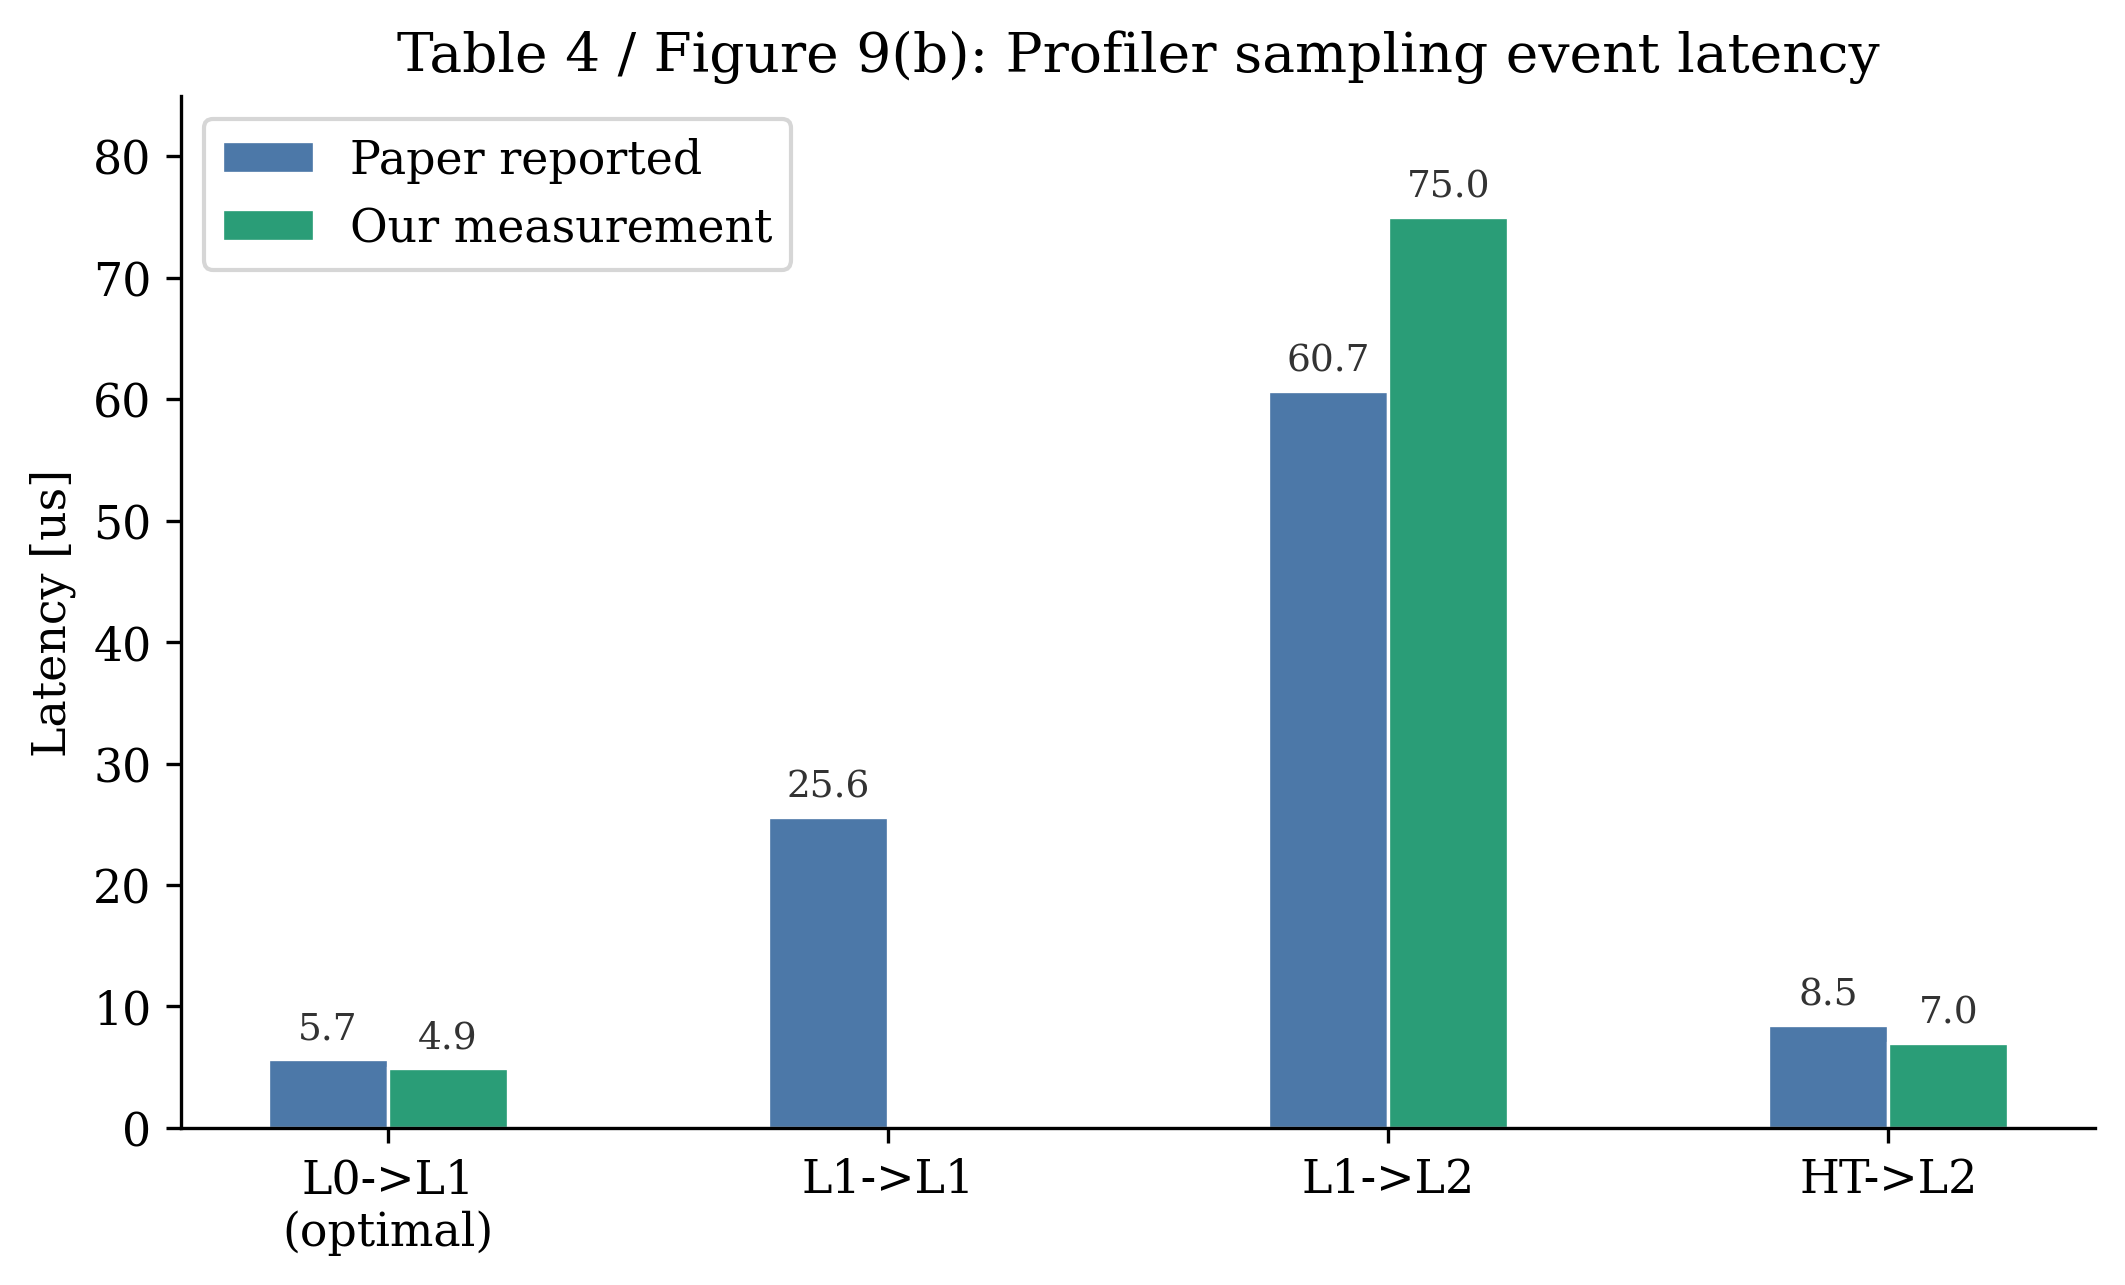
\includegraphics[width=0.55\linewidth]{figures/profiling_sampling_latency.png}
    \caption{Profiler sampling-event handle time (Table~4 / Figure~9b). Three of the four configurations were measured on this stack: L0\,$\to$\,L1 at 4.93\,$\mu$s, L1\,$\to$\,L2 at approximately 75\,$\mu$s, and HT\,$\to$\,L2 at 7.02\,$\mu$s. Only the L1\,$\to$\,L1 entry remains unmeasured.}
    \label{fig:sampling_latency}
\end{figure}

The 1\,kHz Memcached sweep (Figure~\ref{fig:profiling_memcached}) shows a clear separation between the three modes. HyperTurtle profiling stays within 5--17\,$\mu$s of the no-profiling baseline across the 2--20\,Kops/s range, while conventional L1 profiling adds 40--95\,$\mu$s. At 20\,Kops/s, the p99 latency rises from 258.5\,$\mu$s with no profiling to 275.0\,$\mu$s with HyperTurtle and 353.1\,$\mu$s with conventional L1 profiling. A 4\,MiB GUPS-like proxy workload also showed no visible throughput overhead at 1\,kHz in any mode, with all three configurations measuring approximately 310\,Mops across three runs.

\begin{figure}[H]
    \centering
    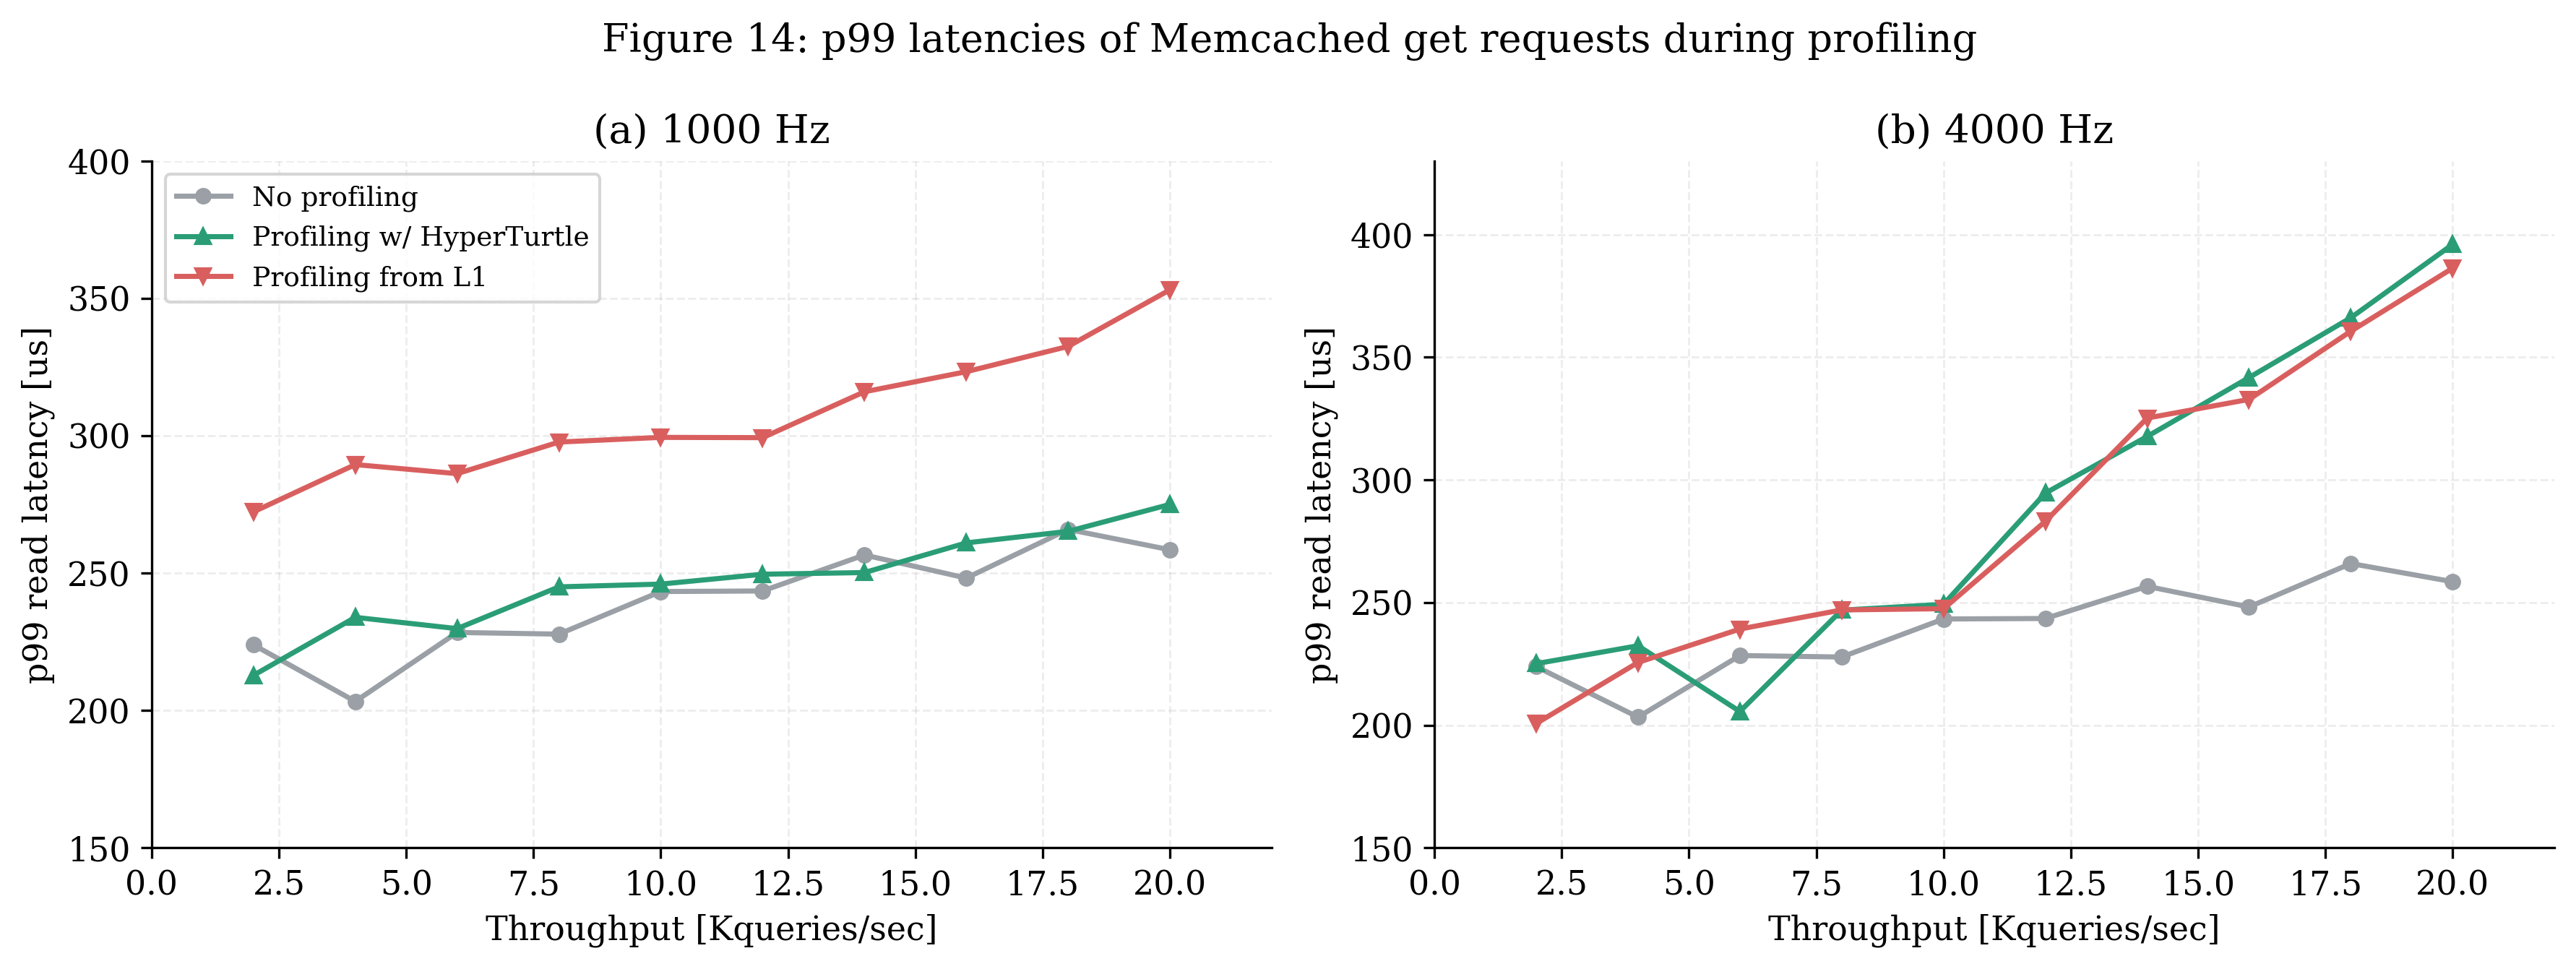
\includegraphics[width=\linewidth]{figures/profiling_memcached_1khz.png}
    \caption{Memcached p99 read latency versus throughput under profiling, measured with \texttt{mutilate} using the Facebook ETC workload distribution. \textbf{(a) 1\,kHz:} HyperTurtle profiling adds only 5--17\,$\mu$s over the no-profiling baseline while conventional L1 profiling adds 40--95\,$\mu$s. \textbf{(b) 4\,kHz:} HyperTurtle and L1 profiling are nearly indistinguishable on this stack, likely because Nested-VirtIO networking caps throughput at $\approx$21\,Kops/s.}
    \label{fig:profiling_memcached}
\end{figure}

At 4\,kHz, HyperTurtle and L1 profiling are nearly indistinguishable on this stack. The most likely cause is the Nested-VirtIO throughput cap at approximately 21\,Kops/s, well below the load range reached by the paper with Direct-Assignment.

\section{Conclusion}

This reproduction validates the paper's three main claims. On EPT, HyperTurtle reduced median nested fault latency from 23.43\,$\mu$s to 5.55\,$\mu$s (4.22$\times$) and improved Kata startup time by 20--33\% across all six images. On networking, HyperTurtle stayed close to the fast path and substantially outperformed the nested baseline on NGINX and Memcached workloads. On profiling, HyperTurtle added only 5--17\,$\mu$s to Memcached p99 latency at 1\,kHz versus 40--95\,$\mu$s for conventional L1 profiling, and the measured HT\,$\to$\,L2 handle time of 7.02\,$\mu$s against 75\,$\mu$s for L1\,$\to$\,L2 gives a 10.7$\times$ speedup consistent with the paper's result.

\end{document}
